
% -*- mode: noweb; noweb-default-code-mode: R-mode; -*-
\documentclass[a4paper]{article}

\title{Sweave Test Document for Heritability by Group}
\author{Joe's BG Temmmam}


\usepackage{a4wide}

\usepackage{Sweave}
\begin{document}

\maketitle
%\usepackage{xtable}
Version: 2011V28;


19+ year-olds with amibiguous sibs and Null values recoded as .375.

\begin{Schunk}
\begin{Sinput}
> x <-rnorm(10)
\end{Sinput}
\begin{Soutput}
 [1]  0.57394270 -0.25282827 -0.97675737 -0.47666520 -0.83738334  1.49374929
 [7]  0.85597354 -0.02435095 -1.17394356  1.51429415
\end{Soutput}
\end{Schunk}


% latex table generated in R 2.14.0 by xtable 1.6-0 package
% Sat Nov 12 13:43:54 2011
\begin{table}[ht]
\begin{center}
\begin{tabular}{rrrrrrrrrrrrrrr}
  \hline
 & $\alpha$ & h\verb|^|2 & c\verb|^|2 & e\verb|^|2 & Mean & SD & Skew &   & .25 & .375 & .5 & .75 & 1 & Total N \\ 
  \hline
Total & 7160 & 0.710 & 0.050 & 0.240 & -0.03 & 1.01 & -0.03 &  & 2206 & 62 & 4864 & 0 & 28 & 7160 \\ 
  All FF & 1782 & 0.850 & 0.040 & 0.120 & -0.04 & 1.02 & 0.04 &  & 574 & 12 & 1186 & 0 & 10 & 1782 \\ 
  All MF & 3558 & 0.650 & 0.060 & 0.290 & 0.01 & 1.02 & -0.06 &  & 1110 & 26 & 2422 & 0 & 0 & 3558 \\ 
  All MM & 1820 & 0.700 & 0.020 & 0.280 & -0.07 & 0.99 & -0.03 &  & 522 & 24 & 1256 & 0 & 18 & 1820 \\ 
   \hline
\end{tabular}
\caption{Height}
\label{tab:two}
\end{center}
\end{table}% latex table generated in R 2.14.0 by xtable 1.6-0 package
% Sat Nov 12 13:43:55 2011
\begin{table}[ht]
\begin{center}
\begin{tabular}{r|rlrc}
  \hline
 & Estimate & Std. Error & z value & Pr($>$$|$z$|$) \\ 
  \hline
(Intercept) & 3.0445 & 0.1709 & 17.81 & 0.0000 \\ 
  outcome2 & -0.4543 & 0.2022 & -2.25 & 0.0246 \\ 
  outcome3 & -0.2930 & 0.1927 & -1.52 & 0.1285 \\ 
  treatment2 & 0.0000 & 0.2000 & 0.00 & 1.0000 \\ 
  treatment3 & 0.0000 & 0.2000 & 0.00 & 1.0000 \\ 
   \hline
\end{tabular}
\end{center}
\end{table}% latex table generated in R 2.14.0 by xtable 1.6-0 package
% Sat Nov 12 13:43:55 2011
\begin{table}[ht]
\begin{center}
{\small
\begin{tabular}{lrrrr}
  & Df & Deviance & Resid. Df & Resid. Dev \\ 
 NULL &  &  & 8 & 10.58 \\ 
   \hline
outcome & 2 & 5.45 & 6 & 5.13 \\ 
  treatment & 2 & 0.00 & 4 & 5.13 \\ 
  \end{tabular}
}
\end{center}
\end{table}

Now we look at Gaussian data:

\begin{Schunk}
\begin{Soutput}
 [1]  0.4750447  0.9506127  1.4138765  0.4904362 -0.5459944 -0.3770295
 [7]  1.2815968 -1.2182136 -0.3996024  0.7517564 -0.5967970 -0.1962042
[13]  2.5385576  0.7041028  1.1901879 -0.4253724 -0.3238622 -1.0783299
[19]  2.0731882 -0.7840216
\end{Soutput}
\begin{Soutput}
	One Sample t-test

data:  x 
t = 1.2594, df = 19, p-value = 0.2231
alternative hypothesis: true mean is not equal to 0 
95 percent confidence interval:
 -0.1960511  0.7884443 
sample estimates:
mean of x 
0.2961966 
\end{Soutput}
\end{Schunk}
Note that we can easily integrate some numbers into standard text: The
third element of vector \texttt{x} is 1.41387654617017, the
$p$-value of the test is 0.22313. % $

Now we look at a summary of the famous \texttt{iris} data set, and we
want to see the commands in the code chunks:



\begin{Schunk}
\begin{Sinput}
> data(iris)
> summary(iris)
\end{Sinput}
\begin{Soutput}
  Sepal.Length    Sepal.Width     Petal.Length    Petal.Width   
 Min.   :4.300   Min.   :2.000   Min.   :1.000   Min.   :0.100  
 1st Qu.:5.100   1st Qu.:2.800   1st Qu.:1.600   1st Qu.:0.300  
 Median :5.800   Median :3.000   Median :4.350   Median :1.300  
 Mean   :5.843   Mean   :3.057   Mean   :3.758   Mean   :1.199  
 3rd Qu.:6.400   3rd Qu.:3.300   3rd Qu.:5.100   3rd Qu.:1.800  
 Max.   :7.900   Max.   :4.400   Max.   :6.900   Max.   :2.500  
       Species  
 setosa    :50  
 versicolor:50  
 virginica :50  
\end{Soutput}
\end{Schunk}


\begin{figure}[htbp]
  \begin{center}
\begin{Schunk}
\begin{Sinput}
> library(graphics)
> pairs(iris)
\end{Sinput}
\end{Schunk}
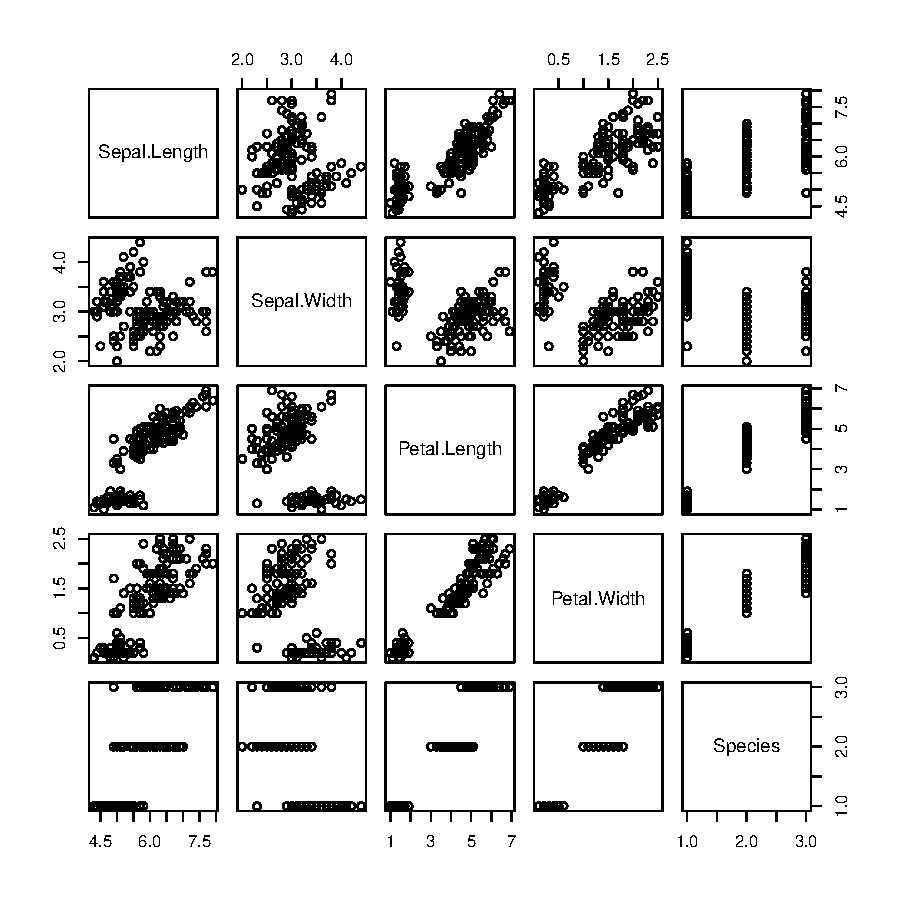
\includegraphics{SweaveTest2-006}
     \caption{Pairs plot of the iris data.}
  \end{center}
\end{figure}

\begin{figure}[htbp]
  \begin{center}
\begin{Schunk}
\begin{Sinput}
> boxplot(Sepal.Length~Species, data=iris)
\end{Sinput}
\end{Schunk}
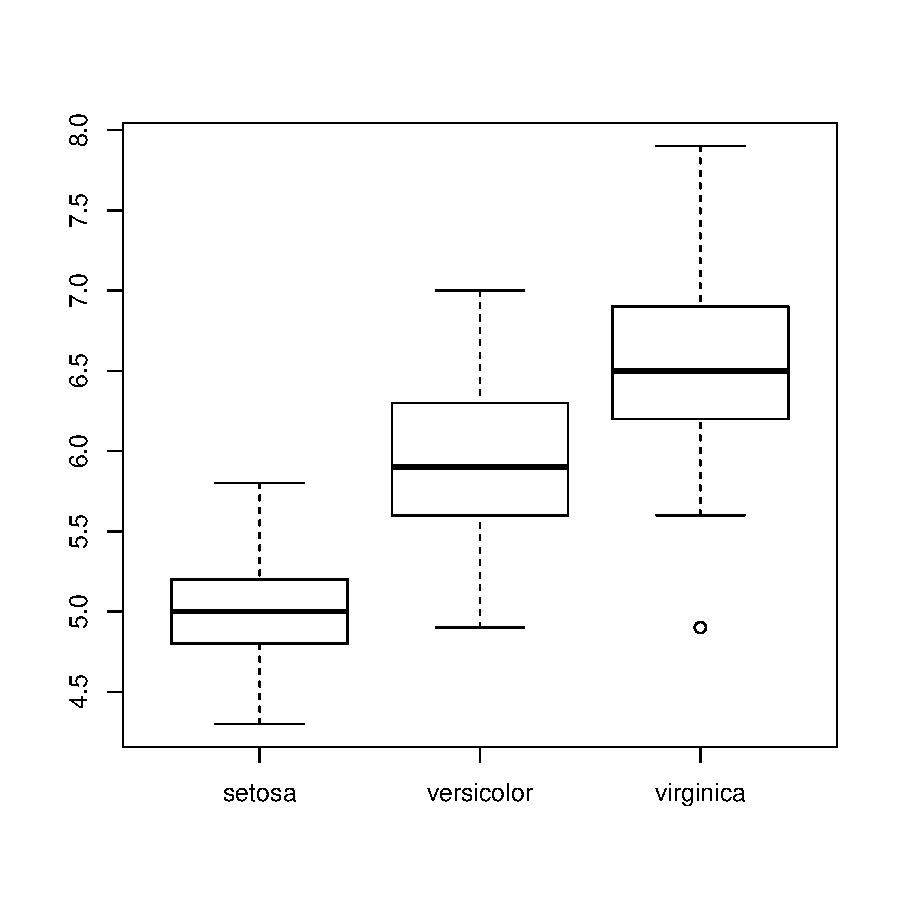
\includegraphics{SweaveTest2-007}
    \caption{Boxplot of sepal length grouped by species.}
  \end{center}
\end{figure}

\end{document}
